\chapter{Architecture and Structural Design}

This chapter details the architectural design of the backtesting engine, justifying the key structural decisions, class methods, and software engineering principles implemented to ensure optimal performance and high scalability.

\section{System Architecture and SOLID Principles}

The system adopts a \textit{Hexagonal Architecture} (Ports and Adapters) to ensure a strict separation of concerns. Following the Dependency Inversion Principle (DIP) of SOLID, the core computational domain does not depend on low-level implementation details (such as data file formats, databases, or external APIs), but rather on abstractions and generic interfaces.

The \textit{Core Domain} exclusively encapsulates the pure financial logic and the vectorized mathematical operations with an asymptotic time complexity of \(\mathcal{O}(1)\). All data ingestion and storage are handled through the \textit{Data Infrastructure}, coupling to the central domain via well-defined ports (such as \texttt{IDataHandler}). This guarantees that the engine can switch between reading data from HDF5 files, Parquet, or a Bloomberg API without modifying a single line of predictive logic.

\section{UML Class Design and Structural Justification}

The structural design focuses on modularity and extensibility, ensuring that each class has a unique responsibility (Single Responsibility Principle - SRP). Figure \ref{fig:class_diagram} illustrates the class hierarchy arranged horizontally for better readability.

\begin{landscape}
\vspace*{\fill}
\begin{figuresrswide}
    \centering
    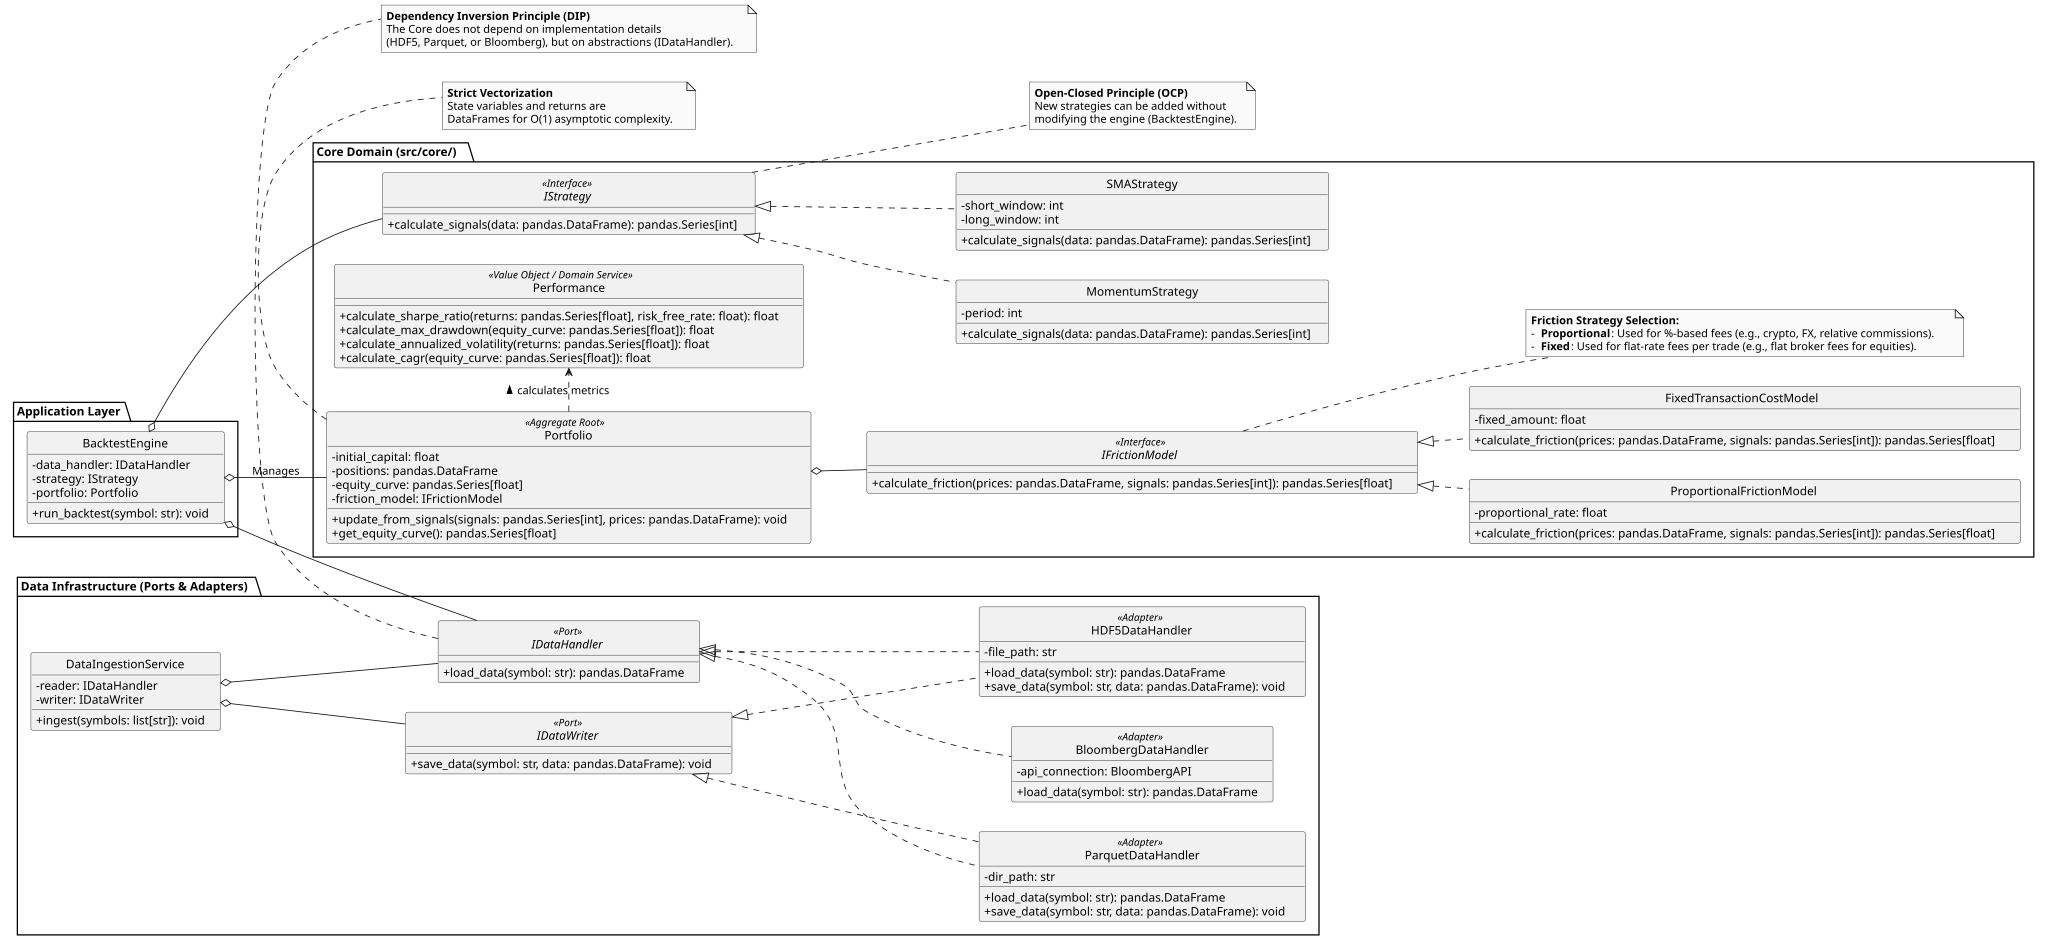
\includegraphics[width=\linewidth,height=14cm,keepaspectratio]{../architecture/class_diagram.pdf}
    \caption{Class Diagram of the Core Architecture}
    \label{fig:class_diagram}
\end{figuresrswide}
\vspace*{\fill}
\end{landscape}
The main components of the system and their fundamental methods span three architectural layers:

\subsection{Application Layer}
\begin{itemize}
    \item \textbf{\texttt{BacktestEngine}}: Acts as the central orchestrator. It encapsulates the injected dependencies (\texttt{IDataHandler}, \texttt{IStrategy}, \texttt{Portfolio}). Its \texttt{run\_backtest(symbol: str)} method coordinates the complete lifecycle: it invokes data loading, passes the \texttt{DataFrame} to the strategy to obtain signals, and delegates state updating and financial calculation to the portfolio.
\end{itemize}

\subsection{Core Domain}
\begin{itemize}
    \item \textbf{\texttt{Portfolio}}: Serves as the Aggregate Root. It maintains immutable state variables in matrix form: initial capital (\texttt{initial\_capital}), holdings (\texttt{positions}), and the value curve (\texttt{equity\_curve}). Its primary method, \texttt{update\_from\_signals(signals, prices)}, crosses trading signals with market returns and applies the injected friction model to generate the historical trajectory. It concludes by exposing the results via \texttt{get\_equity\_curve()}.
    
    \item \textbf{\texttt{IStrategy} and Concrete Strategies}: Base interface defining the pure contract \texttt{calculate\_signals(data) \allowbreak -> Series}. Implementations such as \textbf{\texttt{SMAStrategy}} (with state parameters \texttt{short\_window} and \texttt{long\_window}) or \textbf{\texttt{MomentumStrategy}} (with parameter \texttt{period}) materialize the algorithmic logic. This guarantees the Open-Closed Principle (OCP), allowing the array of strategies to scale without altering the main engine.
    
    \item \textbf{\texttt{IFrictionModel}}: Defines the contract \texttt{calculate\_friction(prices, \allowbreak signals) \allowbreak -> Series} to deduct transactional costs in a vectorized manner. It is materialized in specialized classes like \textbf{\texttt{ProportionalFrictionModel}} (applying a percentage rate, ideal for crypto or Forex) and \textbf{\texttt{FixedTransactionCostModel}} (applying an absolute cost per trade, typical in traditional stock brokerage).
    
    \item \textbf{\texttt{Performance}}: A stateless Domain Service, solely responsible for calculating risk and return metrics from time series. It exposes precise mathematical methods such as \texttt{calculate\_sharpe\_ratio()}, \texttt{calculate\_max\_drawdown()}, \texttt{calculate\_\allowbreak annualized\_\allowbreak volatility()}, and \texttt{calculate\_cagr()}.
\end{itemize}

\subsection{Data Infrastructure (Ports \& Adapters)}
\begin{itemize}
    \item \textbf{\texttt{IDataHandler} and \texttt{IDataWriter}}: Abstract ports defining \texttt{load\_data(symbol)} and \texttt{save\_data(symbol, data)}. They ensure the isolation of the predictive engine from persistence details (Dependency Inversion Principle - DIP).
    
    \item \textbf{Infrastructure Adapters}: Concrete implementations like \textbf{\texttt{HDF5\allowbreak DataHandler}} and \textbf{\texttt{Parquet\allowbreak DataHandler}} for massive hierarchical storage, or \textbf{\texttt{Bloomberg\allowbreak DataHandler}} for real-time or delayed ingestion from external APIs. Additionally, the \textbf{\texttt{DataIngestionService}} orchestrates the iterative fetching and persistence of multiple symbols.
\end{itemize}

\section{Execution Lifecycle}

The orchestration of the simulation follows a unidirectional and deterministic flow, designed to prevent the accidental alteration of state. This can be seen in the Sequence Diagram (Figure \ref{fig:sequence_diagram}).

\begin{figuresrs}
    \centering
    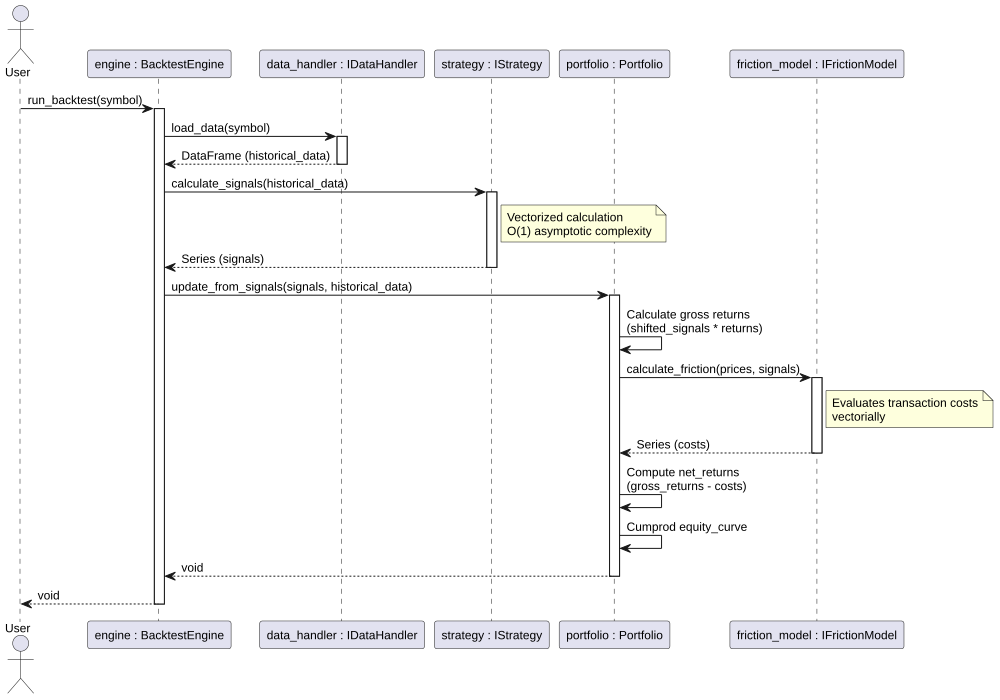
\includegraphics[width=\linewidth,height=17cm,keepaspectratio]{../architecture/sequence_diagram.pdf}
    \caption{Sequence Diagram of the Backtest Execution}
    \label{fig:sequence_diagram}
\end{figuresrs}

The flow is initiated by the user and delegated to the \texttt{BacktestEngine}. This orchestrator retrieves an immutable \texttt{DataFrame} of historical prices via \texttt{load\_data()} from the \texttt{IDataHandler} interface. Subsequently, it passes this structure to the \texttt{IStrategy} abstraction, which evaluates the market and returns an array of signals (e.g., \(+1\), \(0\), \(-1\)). Finally, \texttt{Portfolio} ingests both the prices and the signals in a single matrix operation.

\section{Vectorized Activity Pipeline}

To comply with the strict computational complexity requirement of \(\mathcal{O}(1)\) over massive financial arrays (avoiding any imperative \texttt{for} or \texttt{while} loops), the core of the \texttt{Portfolio} is designed as a purely mathematical conduit. Figure \ref{fig:activity_diagram} details this pipeline.

\begin{figuresrs}
    \centering
    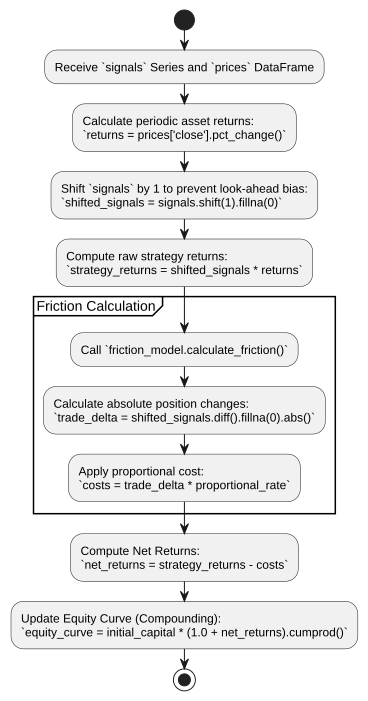
\includegraphics[width=0.6\linewidth]{../architecture/activity_diagram.pdf}
    \caption{Activity Diagram: Vectorized Pipeline in the Portfolio}
    \label{fig:activity_diagram}
\end{figuresrs}
\clearpage
Prior to the algorithmic execution, we establish the foundational mathematical definitions that govern the vectorized operations:

\begin{definition}[Simple Returns]
Let \( P_t \) denote the price of the asset at time \( t \). The discrete percentage return \( R_t \) is calculated as:
\begin{equation}
    R_t = \frac{P_t - P_{t-1}}{P_{t-1}}
\end{equation}
\end{definition}

\begin{definition}[Transaction Friction]
Let \( S_t \in \{-1, 0, 1\} \) be the trading signal at time \( t \) and \( c \) the proportional transaction cost. The friction penalty \( F_t \) incurred at time \( t \) is proportional to the absolute state transition:
\begin{equation}
    F_t = c \cdot | S_t - S_{t-1} |
\end{equation}
\end{definition}

\begin{definition}[Equity Curve]
Given the initial capital \( C_0 \), the strategy signals \( S_{t-1} \) (shifted to avoid look-ahead bias), and the friction \( F_t \), the net return \( \tilde{R}_t \) is \( \tilde{R}_t = S_{t-1} R_t - F_t \). The portfolio value \( E_T \) is defined as the cumulative product:
\begin{equation}
    E_T = C_0 \prod_{t=1}^{T} (1 + \tilde{R}_t)
\end{equation}
\end{definition}

The fundamental algorithmic steps applied to the DataFrame, guaranteeing performance, are:
\begin{enumerate}
    \item \textbf{Returns Calculation:} Native percentage differentiation of the price series.
    \item \textbf{Signal Shifting:} The input signals are mandatorily shifted one time unit forward (\texttt{shift(1)}) to avoid look-ahead bias, ensuring that the investment state at time \(t\) is only executed with the return observed at \(t+1\).
    \item \textbf{Friction Calculation:} The absolute differential of the positions is evaluated through arrays (\texttt{diff().abs()}) to financially penalize only the state transitions, subtracting the associated costs in bulk.
    \item \textbf{Equity Curve:} The continuous cumulative product (\texttt{cumprod()}) is applied to the net returns, achieving the complete evaluation of the historical path in a single native call to the low-level C routines of Pandas/NumPy.
\end{enumerate}
